%template1.tex
%The following LaTeX source file represents the simplest kind of slide presentation; no overlays, no included graphics. Substitute your favorite style for ``pascal''. To create the PDF file template1.pdf, (1) be sure to use the prosper class, then (2) execute the command latex template1.tex, and (3) the command dvipdf template1.dvi.

%%%%%%%%%%%%%%%%%%%%%%%%%%%%%%% template1.tex %%%%%%%%%%%%%%%%%%%%%%%%%%%%%%%%%%%
\documentclass[a4paper,blends,pdf,colorBG,slideColor]{prosper}
% definitions for slides for CSC544
% Lutz Hamel, (c) 2007

\hypersetup{pdfpagemode=FullScreen}

\usepackage{times}
\usepackage{latexsym}
\usepackage{alltt}
\usepackage{booktabs}
\usepackage{amsmath}
\usepackage{amsopn}
\usepackage{amsfonts}
\usepackage{amssymb}
%\usepackage[usenames]{color}

\def\sign{\qopname\relax{no}{sign}}
\def\argmax{\qopname\relax{no}{argmax}}
\def\argmin{\qopname\relax{no}{argmin}}

\newcommand{\grad}{\ensuremath{\nabla}} 
\newcommand{\loss}{\ensuremath{{\cal L}}}
\newcommand{\err}{\mbox{err}}
\newcommand{\mse}{\mbox{mse}}
\newcommand{\acc}{\mbox{acc}}
\newcommand{\Integer}{\ensuremath{\mathbb{N}}}
\newcommand{\size}[1]{{|{#1}|}}
\newcommand{\Rnspace}[1]{\ensuremath{\mathbb{R}^{#1}}}
\newcommand{\Real}{\ensuremath{\mathbb{R}}}
\newcommand{\mytt}[1]{{\small\tt{#1}}}
\newcommand{\textemph}[1]{{\em #1}}
\newcommand{\suchthat}{\mid}
\newcommand{\orbar}{\;|\;}
\newcommand{\bs}[1]{\begin{slide}{#1}\ptsize{8}}
\newcommand{\es}{\end{slide}}
\newcommand{\co}{\,\colon\;}
\newcommand{\pair}[2]{\ensuremath{( {#1}, {#2} )}}
\newcommand{\model}[1]{\hat{#1}}
\newcommand{\ul}[1]{{\bf\em #1}}
\newcommand{\ol}{\overline}
\newcommand{\definition}[1]{{\bf Definition: }{\em #1}}
\newcommand{\example}[1]{{\bf Example: }{#1}}
\newcommand{\abs}[1]{|{#1}|}
\newcommand{\mytab}{\makebox[.1in]{}}

\newcommand{\fdef}[1]{
\begin{center}
\fbox{
\begin{minipage}{3.5in}
{\bf Definition:}
{#1}
\end{minipage}
}
\end{center}
}

\newcommand{\fframe}[1]{
\begin{center}
\fbox{
\begin{minipage}{3.5in}
{#1}
\end{minipage}
}
\end{center}
}

\newcommand{\nframe}[1]{
\begin{center}
\begin{minipage}{3.5in}
{#1}
\end{minipage}
\end{center}
}

\newenvironment{Rcode}
	{
		\scriptsize
		\begin{quote}
		\begin{alltt}
	}
	{
		\end{alltt}
		\end{quote}
	}




\begin{document}

\bs{Multi-Layer ANNs}
The perceptron revisited
\begin{center}
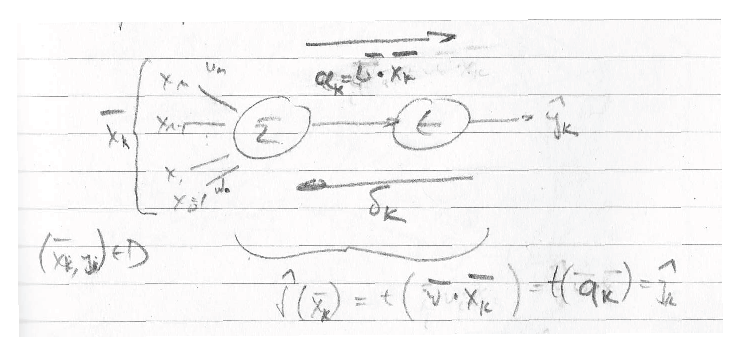
\includegraphics[height=30mm]{images/perceptron-revisited.eps}
\end{center}
Recall
\begin{eqnarray*}
E_k(\ol{w}) &=& \frac{1}{2}(y_k - \model{y}_k)^2\\
	&=& \frac{1}{2}(y_k-t(\ol{w}\bullet\ol{x}_k)^2\\
	&=& \frac{1}{2}(y_k-t(a_k))^2
\end{eqnarray*}
\es

\bs{Multi-Layer ANNs}
We can now look at the gradient,
\begin{eqnarray*}
\grad E_k(\ol{w}) &=& \frac{d}{d\ol{w}} E_k(\ol{w}) \\
	&=& \frac{1}{2} \frac{d}{d\ol{w}}(y_k-t(a_k))^2\\
	&=& -(y_k -t(a_k))\frac{dt}{d\ol{w}}(a_k)\\
	&=& -(y_k -\model{y}_k)\frac{dt}{d\ol{w}}(a_k)\\
	&=& -(y_k -\model{y}_k)\frac{dt}{da_k} (a_k) \frac{da_k}{d\ol{w}} \mbox{ (chain rule)}\\
	&=& -(y_k -\model{y}_k)t'(a_k) \frac{d}{d\ol{w}}(\ol{w}\bullet\ol{x}_k) \\
	&=& -(y_k -\model{y}_k)t'(a_k) \ol{x}_k \\
	&=& \delta_k \ol{x}_k
\end{eqnarray*}
where $\delta_k = -(y_k -\model{y}_k)t'(a_k)$ is called the error.
\es

\bs{Multi-Layer ANNs}
{\bf Observation:} $\grad E_k(\ol{w}) = \delta_k \ol{x}_k$, that is, the gradient at $\ol{x}$ is computed by multiplying the error term $\delta_k$
with the input $\ol{x}$.

\vspace{.1in}

{\bf Observation:} The error term $\delta_k$ is computed by multiplying the observed error $(y_k - \model{y}_k)$ with the derivative 
of the activation function evaluated at $a_k$,
\[
-(y_k -\model{y}_k)t'(a_k)
\]
\es

\bs{Multi-Layer ANNs}
Now recall our update rule,
\[
\ol{w} \leftarrow \ol{w} + \Delta \ol{w}
\]
From before we have
\[
\ol{w} \leftarrow \ol{w} + \eta \grad E_k(\ol{w})
\]
From our discussion above it follows that
\[
\ol{w} \leftarrow \ol{w} + \eta \delta_k\ol{x}_k
\]

\vspace{.2in}
{\bf Observation:} The weights are updated using a scaled version of the input vector.  It is also easy to see that the weights are scaled 
proportional to the error.

This is called {\em back propagation.}

\es
\bs{Multi-Layer ANNs}
\begin{center}
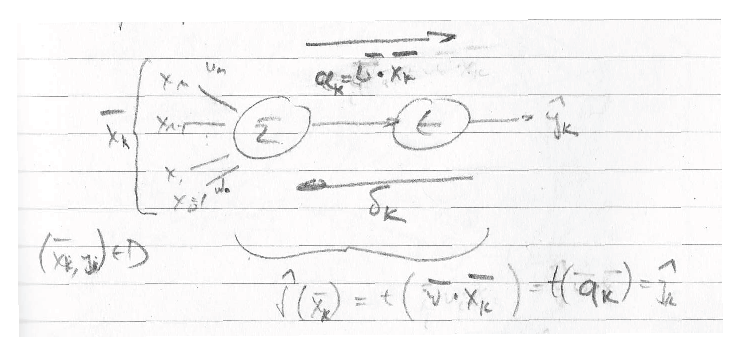
\includegraphics[height=30mm]{images/perceptron-revisited.eps}
\end{center}

Feed forward and backprop neural networks. 
\es

\bs{Multi-Layer ANNs}
A simple ANN with a single hidden layer of $p$ nodes and a differentiable transfer function $t$,

\begin{center}
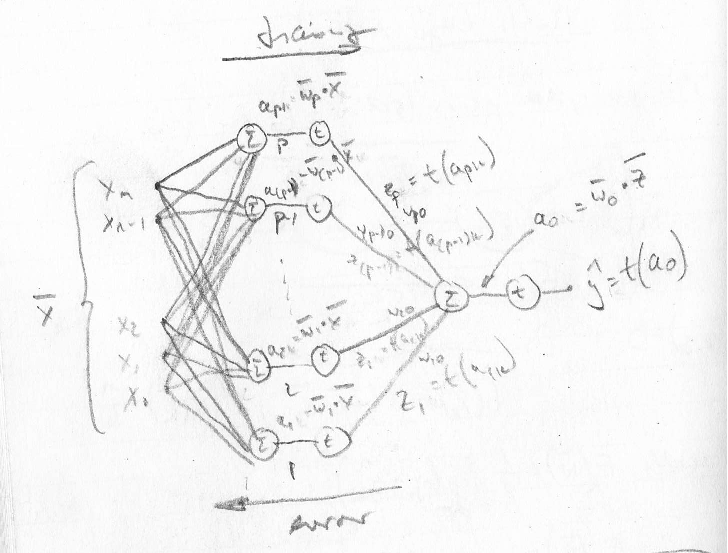
\includegraphics[height=65mm]{images/mlp.eps}
\end{center}

\es

\bs{Multi-Layer ANNs}
How do we train this kind of network?  Observed errors for the hidden layers are no longer available.

\vspace{.2in}
Solution: We systematically backprop the error and use the backprop error instead of the observed error when training the
hidden layer.  
\es

\bs{Multi-Layer ANNs}
Consider a single path through the network:
\begin{center}
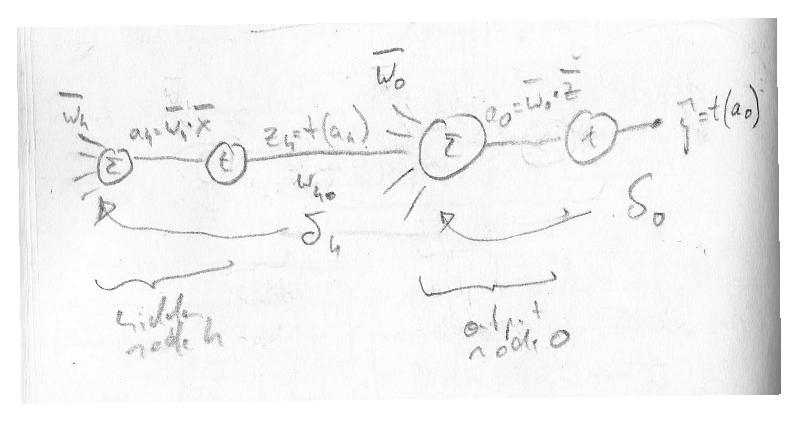
\includegraphics[height=50mm]{images/mlp-single-path.eps}
\end{center}
Training instance $\ol{x}$ is fed forward and the error is back propagated.
\es

\bs{Multi-Layer ANNs}
\small
Now consider the update rule for the weights at the output node $o$,
\[
\ol{w}_o \leftarrow \ol{w}_o + \eta \grad E(\ol{w})
\]
with
\begin{eqnarray*}
\grad E(\ol{w}) &=& \frac{\partial E(\ol{w})}{\partial \ol{w}_o}\\
	&=& \frac{\partial E(\ol{w})}{\partial a_o} \frac{\partial a_o}{\partial \ol{w}_o}\\
	&=& \delta_o \ol{z}
\end{eqnarray*}
where
\[
\frac{\partial a_o}{\partial \ol{w}_o} = \frac{\partial (\ol{w}_o \bullet \ol{z})}{\partial \ol{w}_o} = \ol{z} \mbox{ (see diagram above)
}
\]
and
\[
 \frac{\partial E(\ol{w})}{\partial a_o} = \frac{1}{2} \frac{\partial}{\partial \ol{a}_o} (y - t(a_o))^2 = - (y - t(a_o))t'(a_o) 
= - (y - \model{y})t'(a_o) = \delta_o
\]
This means the update rule for our output node weights becomes,
\[
\ol{w}_o \leftarrow \ol{w}_o + \eta\delta_o \ol{z}
\]

\es

\bs{Multi-Layer ANNs}
\small
Now consider updating the weights for the hidden node $h$,
\[
\ol{w}_h \leftarrow \ol{w}_h + \eta \grad E(\ol{w})
\]
with
\begin{eqnarray*}
\grad E(\ol{w}) &=& \frac{\partial E(\ol{w})}{\partial \ol{w}_h}\\
	&=& \frac{\partial E(\ol{w})}{\partial a_h} \frac{\partial a_h}{\partial \ol{w}_h}\\
	&=& \frac{\partial E(\ol{w})}{\partial a_h} \frac{\partial (\ol{w}_h\bullet\ol{x})}{\partial \ol{w}_h}\\
	&=& \delta_h \ol{x}
\end{eqnarray*}
with
\[
\delta_h = \frac{\partial E(\ol{w})}{\partial a_h} = \frac{\partial E(\ol{w})}{\partial a_o}\frac{\partial a_o}{\partial a_h} = \delta_o \frac{\partial a_o}{\partial a_h} = w_{ho} t'(a_h)\delta_o
\]
Note:
\begin{eqnarray*}
a_o &=& \ol{w}_o \bullet \ol{z} = \ldots + w_{ho} z_h + \ldots = \ldots w_{ho} t(a_h)\dots\\ 
\frac{\partial a_o}{\partial a_h} &=& 0 + \ldots + 0 +w_{ho}t'(a_h)+0+\ldots+0 =w_{ho}t'(a_h)
\end{eqnarray*}

\es

\bs{Multi-Layer ANNs}
Therefore:
\[
\ol{w}_h \leftarrow \ol{w}_h + \eta \delta_h \ol{x} 
\]
or
\[
\ol{w}_h \leftarrow \ol{w}_h +\eta w_{ho} t'(a_h)\delta_o \ol{x}
\]

The updates to the hidden weights is now accomplished with entities that are easily computed.

\vspace{.2in}

Also, since we are stacking neurons we are no longer confined to liner surfaces!  BUT, the error surface is also no longer convex and therefore
a global minimum is much harder to find since there might be lots of local minima.
\es
\end{document}
%%%%%%%%%%%%%%%%%%%%%%%%%%% end of template1.tex %%%%%%%%%%%%%%%%%%%%%%%%%%%%%%%%

